\section{Comparative Annotation Tools}
\label{sec:dataset:architecture_evaluation:tools}

In this section, we describe comparative annotation tools and services used to annotate similar datasets, and compare such tools with Argus.

\subsection{LabelMe} 

LabelMe\footnoteurl{http://labelme.csail.mit.edu/}{17 August 2017} (\cref{fig:dataset:architecture_evaluation:tools:label_me}), developed by \citet{Russell:2008wm}, is a web-based application that requires annotators to set up the web service on their own system. It has been successfully used to markup the large \gls{sun} dataset by novice users, though the developers reflectively note fallbacks and potential difficulties using the tool \citep{DBLP:journals/corr/abs-1210-3448}. LabelMe does not contain a specific instructional workflow, unlike Argus, and therefore annotators are allowed to selectively choose whichever objects to annotate\footnote{Instructions are potentially vague: ``Use your mouse to click around the boundary of \textit{some} objects''.}. This makes the resulting dataset incomplete as (potentially) not all objects in each image are fully annotated. Additionally, there is no restriction to what types of objects are annotated in the image, as any text can be used to describe an object (rather from a hierarchical category, such as in \citep{Lin:2014vma}).

\begin{figure}[h]
  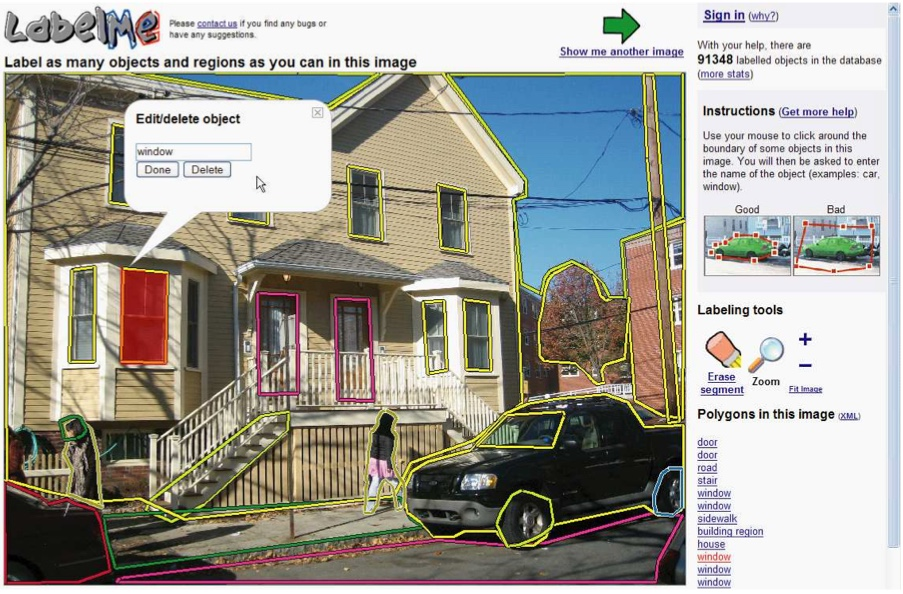
\includegraphics[width=\textwidth]{images/dataset/tools/label_me}
  \caption[The LabelMe user interface]{The LabelMe user interface \citep{Russell:2008wm}.}
  \label{fig:dataset:architecture_evaluation:tools:label_me}
\end{figure}

\subsection{Annotation and Performance Evaluation Platform} 

\citet{Karatzas:2014bt} introduced the \glsac{cvc} \gls{apep}\footnoteurl{http://www.cvc.uab.es/apep/}{17 August 2017}, made popular for use using the \gls{icdar} 2011--2015 Robust Reading Competitions. Unlike our system, users can edit the per-pixel boundaries using a `flood-fill' or `magic-select' markup tool (with an adjustable tolerance), followed by a skeletonisation of the boundaries filled. This speeds up selection of specific text areas (\cref{fig:dataset:architecture_evaluation:tools:apep}). While we did not incorporate a feature into Argus, a potential future version would benefit using such an annotation tool for a polygon, rather than clicking $n_{vertices}$ times if the vertices count is unknown. This could also be encoded using \gls{rle} as suggested from the \gls{coco} format in \cref{sec:dataset:architecture_evaluation}. Additionally, users are able to zoom in to get finer accuracies at the pixel level.


\begin{figure}[h]
  \centering
  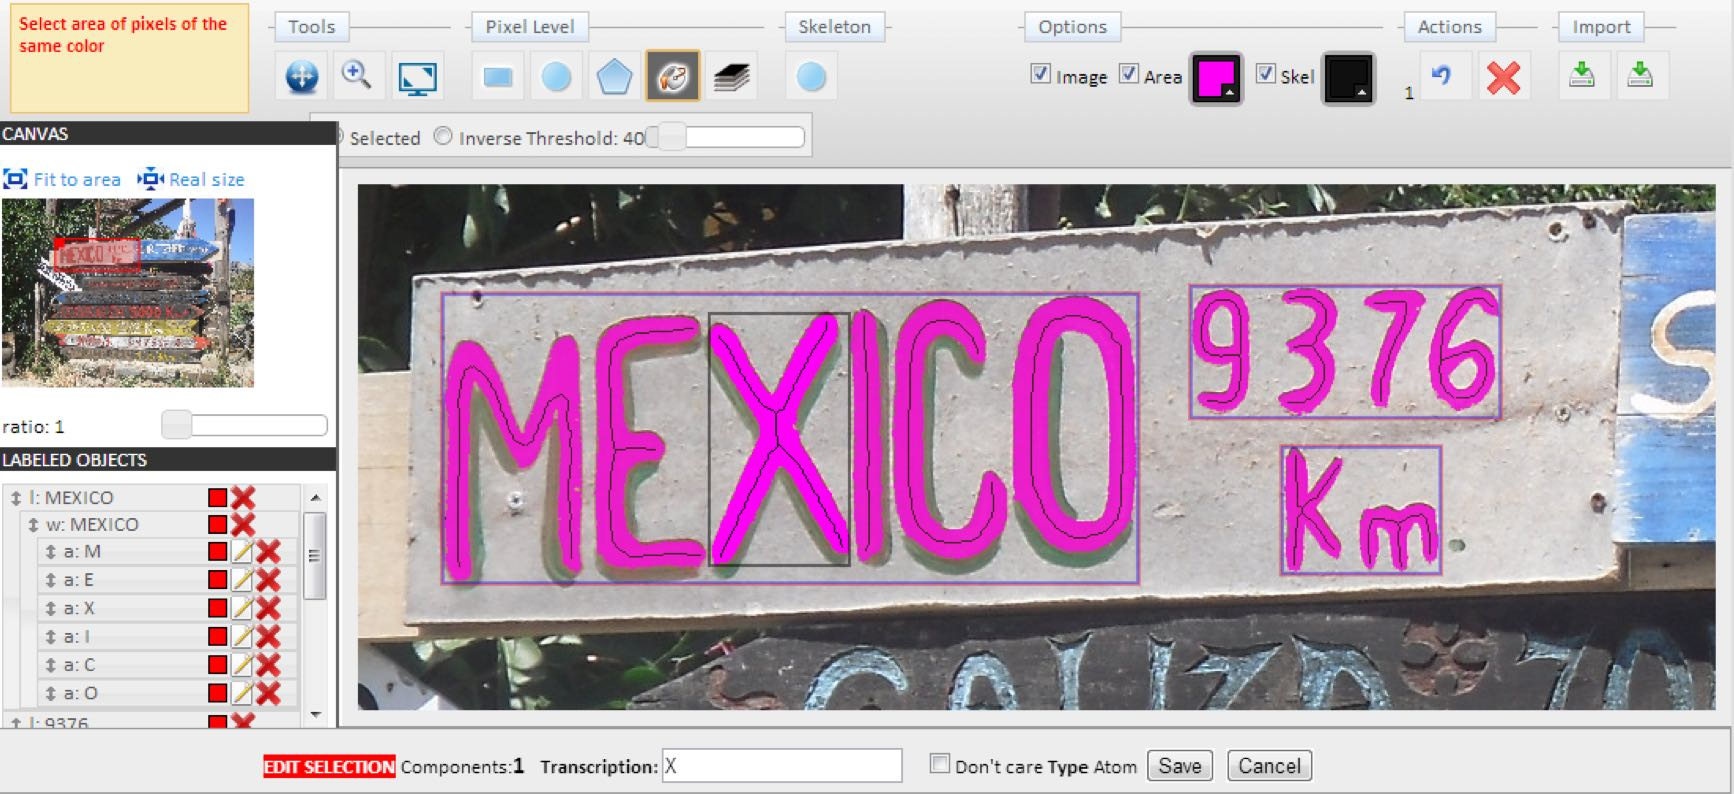
\includegraphics[width=0.9\textwidth]{images/dataset/tools/apep}
  \caption[The APEP user interface]{The APEP ground truth annotation tool, showing a hierachy of textual content and defined text parts (flood-filled areas and skeletons) \cite{Karatzas:2014bt}.}
  \label{fig:dataset:architecture_evaluation:tools:apep}
\end{figure}

% Robust Reading Competition by the Computer Vision Centre: http://www.cvc.uab.es/apep/images/DAS2014_Toolbox.pdf
% ICDAR12-15 which uses CVC Annotation and Performance Evaluation Platform (APEP) \cite{Karatzas:2015tj}

\vspace{-2em}
\subsection{Amazon Mechanical Turk}

\gls{amt}\footnoteurl{https://www.mturk.com/mturk/welcome}{11 August 2017} provides \gls{saas} that does not require downloading or setting up (typically laborious for annotators). Annotation is achieved in the form of customised \glspl{hit}, using a custom-built interface. Recently, this is typically the most popular choice of annotation outsourcing \citep{Lin:2014vma,Veit:2016vj,Chen:2015ur,JiaDeng:2009dl,Netzer:2011to} due to flexibility in developing customised interfaces for the task at hand. The benefits of ensuring a user-friendly crowdsourcing annotation system are presented by \citet{Matera:2014wq}. \citet{Sorokin:2008uk} discuss the utility of using \gls{amt} for annotation. The primary downside is that most interfaces need to be created from scratch, which can typically be laborious.

\subsection{VATIC}

\glsdisp{vatic}{VATIC (the \glsdesc{vatic})} is a a free web-based tool (\cref{fig:dataset:architecture_evaluation:tools:vatic}) developed by \citet{springerlink:10.1007/s11263-012-0564-1}, running on \gls{amt}. We note this tool specifically for the use of annotating video stills within an image: its intended purpose is for the sole use of object tracking in videos. There are only three annotations per object: the object name, the object is out of view, and the object is obstructed. It is useful in that not all frames have to be individually annotated, as the tool uses object tracking to estimate the movement between every 2-3 seconds. This may be useful to incorporate into future works of Argus. 

\begin{figure}[h]
  \centering
  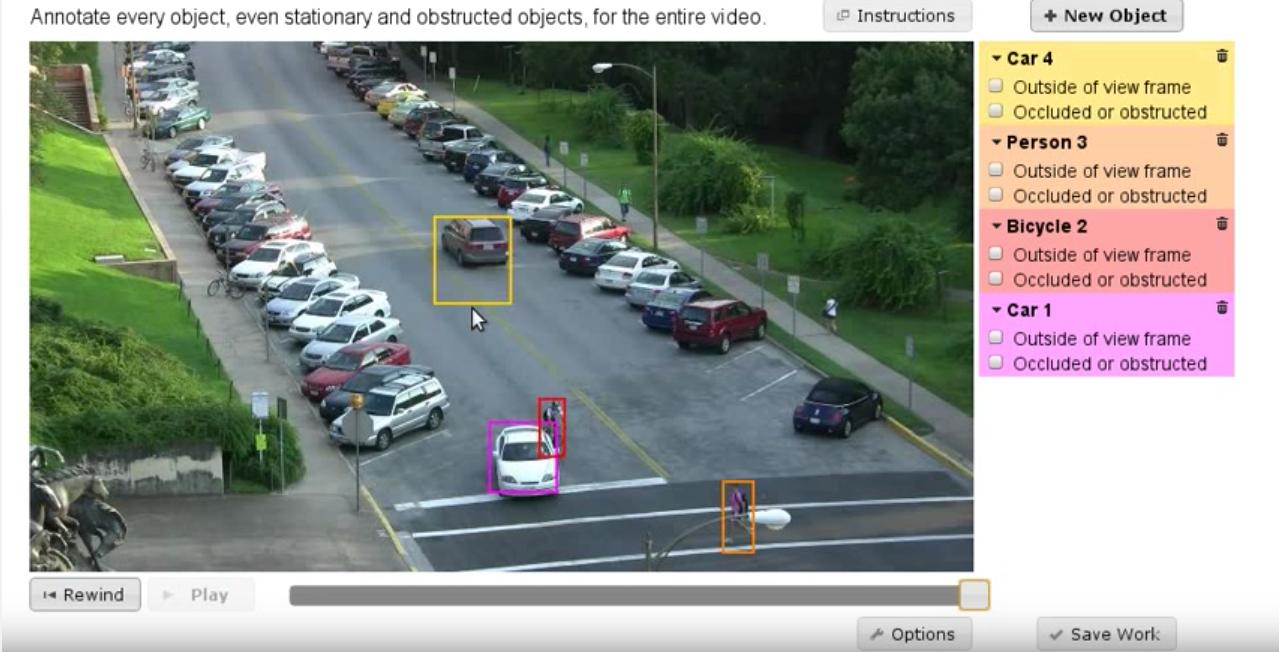
\includegraphics[width=0.9\textwidth]{images/dataset/tools/vatic}
  \caption[The VATIC web-based user interface]{The \gls{vatic} web-based user interface. Sourced from \url{https://github.com/cvondrick/vatic}. (Last viewed 11 August, 2017.)}
  \label{fig:dataset:architecture_evaluation:tools:vatic}
\end{figure}

% - http://carlvondrick.com/vatic/ -> amazon turk
%% Only for object tracking in videos
%% No annotations, only two attributes per feature: (outside view frame or obfuscated)
%% Cannot label each feature, it's Car 1, Car 2, Car 3... may be hard for long videos. 
%% Useful in that you do not need to process every frame
%% PAPER: Utility data annotation with amazon mechanical turk

\vspace{-2em}
\subsection{ScaleAPI}

ScaleAPI\footnoteurl{http://www.scaleapi.com}{11 August 2017} is a recent \gls{saas} that provides a web-based \gls{api} to return human-marked annotation in realtime. Multiple boundary annotations can be made on an image. \cref{lst:dataset:evaluation:scaleapi:req,lst:dataset:evaluation:scaleapi:res} show the request and response for a simple instruction to draw bounding boxes around all pedestrians and cars in the image\footnoteurl{https://docs.scaleapi.com/?shell\#bounding-box-annotation}{17 August 2017}. Additionally, object segmentation (on a per-pixel basis) is provided. While there are no need for workflows in a single request (as multiple requests can be made for multiple workflow steps), instructions to annotators are provided on a per-request basis. This said, a consistent annotator between requests is not guaranteed and this may have an impact on varying annotator quality.

\begin{lstlisting}[language=CURL, label=lst:dataset:evaluation:scaleapi:req, caption={[Sample ScaleAPI request] A sample ScaleAPI HTTP request made using cURL\footnotemark.}]
curl "https://api.scaleapi.com/v1/task/annotation" \
  -u "SCALE_API_KEY:" \
  -d callback_url="http://www.example.com/callback" \
  -d instruction="Draw a box around each **car** and **pedestrian**." \
  -d attachment_type=image \
  -d attachment="http://i.imgur.com/XOJbalC.jpg" \
  -d objects_to_annotate="car" \
  -d objects_to_annotate="pedestrian" \
  -d with_labels=true \
  -d min_width="30" \
  -d min_height="30"  
\end{lstlisting}
\footnotetext{\url{https://curl.haxx.se/} last accessed 17 August 2017.}

\begin{lstlisting}[language=JSON, label=lst:dataset:evaluation:scaleapi:res, caption={[Sample ScaleAPI response] Sample \glsac{json} response from the request made in \cref{lst:dataset:evaluation:scaleapi:req}.}]
{
  "task_id": "5774cc78b01249ab09f089dd",
  "created_at": "2016-9-03T07:38:32.368Z",
  "callback_url": "http://www.example.com/callback",
  "type": "annotation",
  "status": "pending",
  "instruction": "Draw a box around each **car** and **pedestrian**",
  "urgency": "day",
  "params": {
    "with_labels": true,
    "min_width": 30,
    "min_height": 30,
    "objects_to_annotate": [
      "car",
      "pedestrian"
    ],
    "attachment_type": "image",
    "attachment": "http://i.imgur.com/XOJbalC.jpg"
  },
  "metadata": {}
}
\end{lstlisting}
